\chapter{ETUDE DE L’EXISTANT.}     % numéroté chap2
\thispagestyle{fancy}
\definecolor{blue}{RGB}{51,131,255}
\section{État de l’art d’une Marketplace .}

\subsection{Qu’est-ce qu’une Marketplace.}

\begin{enumerate}
		\item  \textbf{Definition}.
		
Le terme de Marketplace, ou place de marché en bon français, désigne toute plateforme qui met en relation des acheteurs et des vendeurs sur Internet. La plateforme récupère en échange une commission sur les ventes qu'elle a permis de réaliser. Certains sites marchands comme eBay ou Rakuten sont des pures Marketplace, c'est-à-dire qu'ils ne proposent que les produits de vendeurs tiers. D'autres, comme Amazon, Cdiscount ou Rueducommerce, accueillent les produits de ces vendeurs tiers, aux côtés de leur propre gamme de produits\cite{Ref3}.
		
Ces vendeurs, qui sont parfois même des particuliers, profitent alors des fonctionnalités de la plateforme d'e-commerce et de son audience. Autrement dit et de manière schématique, une Marketplace, c'est comme un centre commercial, mais sur Internet. La place de marché propose en effet une sorte de galerie marchande digitale dédiée aux vendeurs. Ces derniers y installent leur propre magasin en ligne et y font leurs affaires. Le marchand qui gère la Marketplace peut, dans certains cas, leur proposer de prendre en charge le stockage et l'expédition des produits. Le vendeur doit lui faire appel à un gestionnaire de flux pour gérer la diffusion de son catalogue produit au sein de la Marketplace, suivre ses ventes et ajuster sa stratégie en conséquence.

A la base, l'intérêt de la Marketplace était de servir d'intermédiaire dans une relation interprofessionnelle (B2B). Quand le client peut payer en ligne sur la Marketplace. Aujourd'hui, cette technique s'est ouverte au B2C via des sites marchands gigantesques. 

Au regard de tout ce qui précède, IZIWAY ambitionne de se doter de nombreux outils qui sera intégré à son application mobile et devra améliorer l’utilisation de son application et aussi de fidéliser ses clients.

		
		\item \textbf{Les acteurs de la marketplace} 
		
Dans un Marketplace on distingue trois acteurs principaux acteurs et d’autres secondaires, qui ont des rôles spécifiques et complémentaires afin de concrétiser une vente. 

\begin{figure}[H]
	\centering
	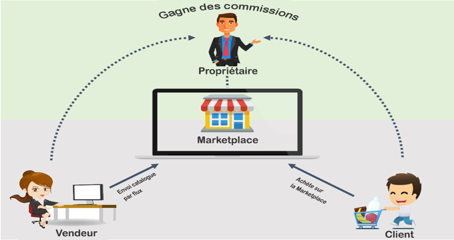
\includegraphics[width=13cm]{acteurs.png}
	\caption{Acteurs de la marketplace}{ \begin{center} source : \textit{https://www.redsen-consulting.com/fr/inspired/marketplace/marketplace-les-acteurs-secondaires} \end{center}}
	\label{fig:acteurs}
\end{figure}

\item \textbf{Typologie des relations commerciales } 

Les entreprises et les consommateurs sont les deux acteurs plus courts au commerce électronique. Il existe quatre types principaux\cite{Ref12} :

\begin{itemize}[label=\textbullet, font=\LARGE \color{blue}]
	\item La Marketplace B2C (Business to Consumer) : elle est destinée aux transactions ou mises en relations entre vendeurs professionnels et acheteurs particuliers . C’est aujourd’hui la forme la plus connue de la Marketplace avec des acteurs comme Amazon, Cdiscount. Un des facteurs clés de succès de la Marketplace B2C est basé sur les volumes que celle-ci a su drainer.
	\item La Marketplace B2B (Business to Business) : commerce électronique entre des entreprises, elle est plus ancienne que B2C
	\item La Marketplace C2B (Consumer to Business) : commerce électronique dont un consommateur est au service de l’entreprise, comme appels d’offres d’emplois d’un projet.
	\item La Marketplace C2C (Consumer to Consumer) : commerce électronique entre deux consommateurs sur des sites qui offrent des annonces sur internet, ou peut-être même deux particuliers peuvent vendre et acheter en ligne.
\end{itemize}

\item \textbf{Les cinq paliers de la Marketplace}

 Une Marketplace efficace repose sur cinq piliers nécessaires : \cite{Ref5}
 
 \begin{itemize}[label=\textbullet, font=\LARGE \color{blue}]
	\item Le trafic : est le palier le plus important dans une Marketplace, car cette dernière est en relation directe avec le trafic, plus il y’a des visiteurs plus les opportunités de transactions seront nombreux et la visibilité des articles des vendeurs augmente.
	\item Le mix produit : on peut distinguer deux types de Marketplace :
		\begin{itemize}[label=\textbullet, font=\LARGE \color{black}]
			\item Des Marketplace avec une faible limite imposé aux vendeurs et la restriction des quasi-inexistant, le vendeur peut poser tous types d’articles
			\item Des Marketplace ou les opérateurs définissent précisément quels produits mis en vente avec une maitrise de catalogue, chaque article doit respecter le catalogue qui lui convient.
		\end{itemize}
	\item Le cadre légale : les Marketplace n’imposent pas le même niveau d’exigence au niveau juridique. Pour certains Marketplace les contrats sont bien contrôler pour les échanges des articles sensibles. Et pour d’autres cette exigence est moindre, l’identification des intervenants n’est pas trop poussé.
	\item Les outils de communication et de la gestion de cycle de vente : 
		\begin{itemize}[label=\textbullet, font=\LARGE \color{black}]
			\item Les outils de communication entre les acheteurs et les vendeurs sont les facteurs les plus importants de la réussite de concrétisation d’une vente et de l’après-vente, sa peut être des messageries, chat, et beaucoup d’autres outils.
			\item Pour la gestion du cycle de vente, les Marketplace affichent aux vendeurs la quantité de stocks de ses produits mise à jour au temps réel. Ainsi que les opérateurs suivent les transactions d’achat avec tous les états d’avancement de la commande jusqu’à la réception de l’article par le client.
		\end{itemize}
	\item Le paiement : cette partie est très sensible, elle doit être bien contrôlée, pour avoir la confiance du client. Il faut leur assure que les opérateurs enregistrent la transaction dans un environnement sécurisé, et que leurs données sont bien protégées.
\end{itemize}
\end{enumerate}

\subsection{Avantages et inconvénients d’une Marketplace }

Il faut bien connaître les avantages et inconvénients de la Marketplace par rapport aux deux principaux acteurs, l’entreprise et le client :
\begin{enumerate}
	\item  \textbf{Avantages}.
	
	Pour l'entreprise : 
\begin{itemize}[label=\textbullet, font=\LARGE \color{blue}]
	\item Permet d’envisager la politique de la fidélisation du client à travers une offre des services.
	\item Nouveau canal de distribution qui permet de se développer sur le marché mieux qu’un magasin physique.
	\item Meilleure économie en évitant les coûts des locaux, des magasins.
	\item Améliorer la visibilité des produits, donc c’est un marketing très efficace.
	\item Permet de toucher des nouveaux clients et développer une relation entre eux et l’entreprise.
\end{itemize}
	Pour le client : 
\begin{itemize}[label=\textbullet, font=\LARGE \color{blue}]
	\item Plus de choix des produits et avec des prix moins chers
	\item Économie de temps puisque le client peut acheter sans se déplacer.
	\item Un renseignement sur la qualité de produit grâce aux descriptions bien détaillées.
	\item Des économies grâce à la possibilité de comparer les prix.
	\item Possibilité d’acheter n’importe où et à n’importe quelle heure (24h/24 et 7j/7)
	\item Pas de file d’attente
	\item Shopping de la maison 
\end{itemize}
	\item  \textbf{Inconvénients}.
	
	Pour l'entreprise : 
\begin{itemize}[label=\textbullet, font=\LARGE \color{blue}]
	\item L’insécurité des transactions et le manque de confiance des moyens de paiements face aux pirates.
	\item Des frais supplémentaires ou la nécessité d’une bonne formation du personnel
	\item L’anonymat du client
	\item Coût de la logistique plus élevée que le commerce classique comme les frais de transports.
\end{itemize}
	Pour le client : 
\begin{itemize}[label=\textbullet, font=\LARGE \color{blue}]
	\item L’insécurité de paiement et la possibilité de tomber sur des sites malveillants.
	\item En cas de problème c’est difficile de contacter le service après-vente
	\item Le manque de contact avec le produit et par la suite le client ne peut pas bien se rendre compte sur ses qualités et ses défauts
	\item Absence de contact avec le vendeur et par la suite le manque de conseils.	
\end{itemize}
\end{enumerate}

\section{Description de l'existant.}

\subsection{Type de marketplace}

IZIWAY est une plateforme de e-commerce 100\% camerounaise qui a été lancé en décembre 2019. Pour son lancement il a été question pour le promoteur de la plateforme de savoir sur quel business model \cite{Ref6}. Soucieux de faire du chiffre d’affaire et de satisfaire notre clientèle, IZIWAY a décidé d’utiliser le model B2C (Business to Consumer) qui est aujourd’hui le model le plus utilisé dans le monde.

De nos jours beaucoup d’entreprises effectuent l’achat de leurs matériels en ligne, il est donc question pour nous de les avoir dans notre portefeuille. C’est dans cette optique que IZIWAY est entrain de migrer vers un business model hybride c’est-à-dire qu’il va être du B2C (Business to Consumer) et du B2B (Business to Business). Ce modèle hybride va nous permettre d’avoir une clientèle large qui peut être à la fois des personnes physiques ou des entreprises.

\subsection{Présentation de l’existant}

Nous allons présenter la procédure allant de l’achat d’un article par un client jusqu’à sa livraison. Cette procédure s’applique à toute plateforme de e-commerce. 
\begin{figure}[H]
	\centering
	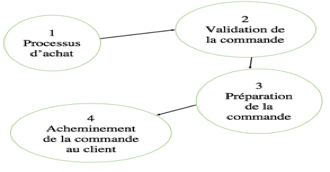
\includegraphics[width=13cm]{processuspassation.png}
	\caption{Processus de passation d'une commande}{ \begin{center} source : \textit{https://www.joelpro-educ.com/s/passation-de-la-commande-2nde-stt-cours} \end{center}}
	\label{fig:processus}
\end{figure}

La description de la figure ci-dessus est capitale pour une bonne compréhension de la situation.
\begin{enumerate}
	\item  \textbf{Proposition d'achat :} étape au cours de laquelle un client fait une recherche du produit qu’il veut, valide son produit et effectue son achat..
	\begin{itemize}[label=\textbullet, font=\LARGE \color{blue}]
		\item La recherche : ici le client parcourt l’application et utilise le module de recherche afin de découvrir les produits disponibles,
		\item La validation sociale : appelée ‘Social Proof’ en anglais, elle fait référence à la consultation d’avis clients sur le produit par le client	
		\item L’ajout au panier : l’internaute peut choisir de poursuivre ses recherches et ajouter d’avantages de produits ou bien de s’arrêter là,
		\item La création d’un compte 
		\item Le renseignement des données de facturation et de livraison 
		\item La sélection du mode livraison : à domicile, retrait en agence
		\item La sélection du moyen de paiement : par transaction bancaire, par Orange Money/ Mobile Money, par paiement à la livraison 
		\item La confirmation de l’achat : le client a terminé sa commande.
	\end{itemize}
	\item  \textbf{La Validation de la commande :} étape au cours de laquelle le client est contacté par le service client qui lui remémore sa commande avec les différents prix et lui demande s’il veut valider la commande.
	\item  \textbf{Préparation de la commande :} ici le service client appelle le vendeur pour qu’il vienne déposer l’article contre une décharge. Lorsque le vendeur dépose l’article le service de la logistique prépare l’article en emballant le produit.
	\item  \textbf{Acheminement de la commande au client  :} Ici le service de livraison appelle le client pour lui faire comprendre que son article est déjà prêt et qu’un livreur est en chemin pour le livrer.
\end{enumerate}

\subsection{Critique de l'existant.}

 D’entrée de jeu, nous avons créé un sondage que nous avons mis à la disposition de notre clientèle afin de collecter un maximum d’idées nouvelles sur notre hypothèse. Après notre investigation avec l’aide de Pareto\cite{Ref8}, nous avons constaté de nombreux problèmes relevés par nos différents utilisateurs. Parmi les problèmes relevés lors de notre côtoiement du métier nous pouvons énumérer les plus pertinents :
 
\begin{itemize}[label=\textbullet, font=\LARGE \color{blue}] 
	\item Ergonomie peu désirable :  En effet la première chose qu’un utilisateur remarque sur une application c’est son côté artistique, la beauté de l’application.
	\item Le manque de notification sur l’application : Les notifications sur une application sont primordiales parce qu’elles permettent à l’opérateur de mettre les utilisateurs des nouveaux deals qui se préparent
	\item Le manque de changement des produits sur la page d’accueil de l’application 
	\item La mise à jour récurrente de l’application 
	\item Recherche peu conviviale
\end{itemize}


\section{Cahier de charge .}

\subsection{Definition du projet.}

Aujourd’hui, toutes les entreprises qui veulent progresser dans un environnement concurrentiel doivent se doter d’un système d’information fiable. Le système d’information est un ensemble organise de ressources qui permet de collecter, stocker, traiter et distribuer de l’information. Il s’agit d’un système sociotechnique compose de deux sous-systèmes, l’un social et l’autre technique : 

\begin{itemize}[label=\textbullet, font=\LARGE \color{blue}] 
	\item Le sous-système social est composé de la structure organisationnelle et des personnes liées au SI,
	\item Le sous-système technique est composé des technologies (hardware, software et équipements de télécommunication) et des processus métiers concernés par le SI.
\end{itemize}

Afin de bénéficier d’un SI fiable et compétitif, les entreprises utilisent l’informatique comme socle de leur SI afin de bénéficier d’une circulation et d’un traitement rapide des informations pour une meilleure exploitation.

C’est dans ce cadre que nous devons améliorer une infrastructure informatique fiable et compétitive dans leur SI pour le processus d’achat des articles et l’aisance de plus de 10000 utilisateurs, afin de disposer de fidèle client.

\subsection{Présentation des concurrents .}

Le commerce sur Internet est dominé par les deux géants américains Amazon et eBay. Nombreux sont les internautes qui se déplacent directement sur ces deux plateformes de vente pour effectuer leurs achats. Néanmoins en Afrique le leader du e-commerce est Jumia. Il est conseillé de s’intéresser également aux autres Marketplace en ligne, car elles peuvent représenter des opportunités séduisantes (et ce en particulier pour les petites et moyennes entreprises). Nous pouvons citer entre autre :

\begin{itemize}[label=\textbullet, font=\LARGE \color{blue}] 
	\item AMAZON : Le géant Amazon s’est lancé en 1994 en tant que libraire en ligne pour ensuite se diversifier et devenir un énorme centre logistique. L’entreprise américaine propose une palette assez large et spécialisée de ses propres produits, des services en ligne mais donne surtout la possibilité aux entreprises du monde entier de commercialiser leurs produits sur sa Marketplace. 
		\begin{figure}[H]
			\centering
			
\includegraphics[width=5cm]{amazon.png}
			\caption{Amazon.}{ \begin{center} source : \textit{Google} \end{center}}
			\label{fig:amazon}
		\end{figure}
	Nous pouvons avoir les avantages suivants :
	\begin{itemize}[label=\textbullet, font=\LARGE \color{black}] 
		\item Fort trafic
		\item Nombreuses interfaces	
		\item Logistique possible via Amazon
		\item Possibilité de faire de la publicité pour son offre (payant)
	\end{itemize}
	Comme inconvénients nous pouvons avoir  :
	\begin{itemize}[label=\textbullet, font=\LARGE \color{black}] 
		\item Forte concurrence
		\item Frais élevés 	
		\item Impossible de créer son propre design
	\end{itemize}
	
	\item ALIBABA : Le groupe chinois Alibaba est représenté en ligne sur plusieurs places de marché : en plus de Alibaba.com (une plateforme B2B) et Taobao (une plateforme de vente similaire à eBay), l'entreprise a également un marché en ligne pour le B2C dans son portefeuille avec AliExpress. Sur AliExpress, les clients peuvent faire des achats dans le monde entier, mais les vendeurs eux-mêmes sont tous chinois. Les autres marchands en ligne ne sont pas autorisés à proposer leurs produits sur la plateforme de vente. Il en va différemment pour la filiale éponyme : les commerçants internationaux peuvent trouver des clients dans le monde entier.
		\begin{figure}[H]
			\centering
			
\includegraphics[width=5cm]{alibaba.png}
			\caption{Alibaba.}{ \begin{center} source : \textit{Google} \end{center}}
			\label{fig:alibaba}
		\end{figure}
		Nous pouvons avoir les avantages suivants :
	\begin{itemize}[label=\textbullet, font=\LARGE \color{black}] 
		\item Fort trafic
		\item Pages d'articles peronnalisables	
		\item Marche international
		\item Option (payante) de promotion des annonces
		\item pas de commissions sur les ventes
		\item Logiciel specifique pour faciliter les vente
	\end{itemize}
	Comme inconvénients nous pouvons avoir  :
	\begin{itemize}[label=\textbullet, font=\LARGE \color{black}] 
		\item Forte concurrence
		\item Frais élevés 	
		\item La traduction francaise laisse parfois à desirer
	\end{itemize}
	
	\item JUMIA : est une entreprise de commerce électronique presente sur le marché africain et fondée en 2012. En 2019, plus de 80 000 vendeurs proposent une large gamme de produits et de services à la demande : appareils électroménagers et électroniques, mode, jouets pour enfants mais aussi des services tels des réservations d'hôtels ou d’avion, et la livraison de repas. Jumia est notamment qualifié d'« Alibaba africain » ou d'« Amazon africain ».
		\begin{figure}[H]
			\centering
			
\includegraphics[width=5cm]{jumia.png}
			\caption{Jumia.}{ \begin{center} source : \textit{Google} \end{center}}
			\label{fig:jumia}
		\end{figure}
		Nous pouvons avoir les avantages suivants :
	\begin{itemize}[label=\textbullet, font=\LARGE \color{black}] 
		\item Fort trafic
		\item Propre boutique jumia et conception de la mise en page possible	
		\item Nombreuses interfaces
		\item Possibilité de faire la publicité pour son offre (payant)
	\end{itemize}
	Comme inconvénients nous pouvons avoir  :
	\begin{itemize}[label=\textbullet, font=\LARGE \color{black}] 
		\item Forte concurrence
		\item Connexion à paypal pas très sécurisé 	
	\end{itemize}
	
\end{itemize}

\subsection{Caractéristiques de la solution voulue :}

\begin{table}[H]
	\caption{Caractéristiques de la solution voulue}
	\label{Caractéristiques de la solution voulue}
	\centering
	\begin{tabularx}{\linewidth}{|X|X|X|}
		\hline \rowcolor{lightgray}  
		\textbf{Objectif} & \textbf{Définition} & \textbf{Comment?}\\
		\hline
		Fiabilité & Assurer l'authenticité des informations &  En connectant l'application à une base de données sql server qui contient au préalable des informations\\
		\hline
		Intégrité & Assurer l'authenticité de l'application c'est à dire la non modification possible du contenu et la forme &  En donnant les droits de modifications a l'administrateur juste\\
		\hline
		Sécurité & Assurer la sécurité des informations & Le personnel n'a pas accès a l'application sauf les responsables des différentes équipes\\
		\hline
		Evolutivité  & Permettre l'actualisation des informations par rapport personnel &  Apres le test de l'application, nos sommes a l'écoute des remarques de la Direction des Ressources Humaines \\	
		\hline
		
	\end{tabularx}
\end{table}

\subsection{Spécification des besoins :}

Cette phase consiste à comprendre le contexte du système. Il s’agit de déterminer les fonctionnalités et les acteurs les plus pertinents, de préciser les risques les plus critiques.

\textbf{Besoins fonctionnels}

L’amélioration qui doit être effectuée sur l’application se veut d’être opérationnel, évolutif, convivial et offrant les informations nécessaires à temps réel.

Pour ceci, le système à réaliser doit satisfaire les exigences de la totalité des utilisateurs. Nous présenterons dans ce qui suit tous les besoins fonctionnels classés par acteurs ainsi que les besoins non fonctionnels communs à tous ces acteurs.

Un acteur est une personne, un matériel ou un logiciel qui interagit avec le système dans le but de réaliser une plus-value.

Les principaux acteurs en interactions avec notre système sont :

	\begin{itemize}[label=\textbullet, font=\LARGE \color{blue}] 
		\item L'informaticien
		\item Le responsable marketing	
		\item Le responsable content-writer
		\item Le client
		\item Le responsable de la planification commercial
	\end{itemize}
	
	Les besoins fonctionnels classés par acteur :
	
	\begin{itemize}[label=\textbullet, font=\LARGE \color{blue}] 
		\item Le responsable marketing
			\begin{itemize}[label=\textbullet, font=\LARGE \color{black}] 
				\item Créer les push notifications
			\end{itemize}
		\item Le responsable content-writer
			\begin{itemize}[label=\textbullet, font=\LARGE \color{black}] 
				\item Créer et modifier les sliders
				\item Créer et modifier les doubles bannières
			\end{itemize}
		\item L'informaticien
			\begin{itemize}[label=\textbullet, font=\LARGE \color{black}] 
				\item Faire la maintenance de l'application
				\item Faire le paramétrage de l'application
				\item Faire le suivi
			\end{itemize}
		\item Le client
			\begin{itemize}[label=\textbullet, font=\LARGE \color{black}] 
				\item Effectué un achat 
				\item Consulter les différents produits disponibles, les différents sliders et les différentes bannières
			\end{itemize}
		\item Le responsable de la planification commercial
			\begin{itemize}[label=\textbullet, font=\LARGE \color{black}] 
				\item Ajouter et modifier le bloc produits et le bloc catégori
			\end{itemize}
	\end{itemize}
	
\textbf{Besoins non fonctionnels}


A part les besoins fondamentaux, notre système doit répondre aux critères suivants :


\begin{itemize}[label=\textbullet, font=\LARGE \color{blue}] 
	\item La rapidité de traitement : En effet, vu le nombre important des transactions quotidiennes, il est impérativement nécessaire que la durée d’exécution des traitements s’approche le plus possible du temps réel,
	\item  La performance : une application doit être avant tout performant c’est-à-dire à travers ses fonctionnalités, répond à toutes les exigences des usagers d’une manière optimale,
	\item  La convivialité : l’application doit être facile à utiliser. En effet, les interfaces utilisateurs doivent être conviviales c’est-à-dire simple, ergonomiques et adaptées à l’utilisateur.
	
\end{itemize}

\subsection{Solutions envisageables.}

L’informatique en entreprise peut être gérée de deux façons :

\begin{itemize}[label=\textbullet, font=\LARGE \color{blue}]
	\item  \textbf{L’externalisation:} c’est le principe selon lequel une entreprise confie à un prestataire extérieur, 	
	\item  \textbf{L’internalisation }  l’entreprise s’occupe elle-même de la gestion de son système d’information en interne.
\end{itemize}

Chacune des deux méthodes présente des avantages et inconvénients que nous allons présenter par la suite.

\textbf{\underline{L'externalisation.}}

\begin{table}[H]
	\caption{Avantages et inconvénients de l'externalisation}
	\label{Avantages et inconvénients de l'externalisation}
	\centering
	\begin{tabularx}{\linewidth}{|X|X|}
		\hline \rowcolor{lightgray}  
		\textbf  \textbf{Avantages} & \textbf{Inconvénients}\\
		\hline
		 Ouverture de l'entreprise sur l'extérieur : la coopération est une démarche enrichissante &  Choc culturel engendré par la venue de nouveaux collaborateurs salariés du prestataire\\
		\hline
		Concentration sur le coeur métier dans une logique de spécialisation &  Crainte d'un backsourcing impossible ou d'un changement de prestataire\\
		\hline
		 Concentration sur le coeur de métier dans une logique de spécialisation  & perte de confidentialité \\
		\hline
		 Gain de réactivité de l'entreprise &  risque de mésentente entre le prestataire et le client \\	
		\hline		
	\end{tabularx}
\end{table}{  source : \textit{https://www.petite-entreprise.net/P-2555-81-G1-avantages-et-inconvenients-de-l-externalisation.html}

\textbf{\underline{L'internalsiation.}}

\begin{table}[H]
	\caption{Avantages et inconvénients de l'internalisation}
	\label{Avantages et inconvénients de l''internalisation}
	\centering
	\begin{tabularx}{\linewidth}{|X|X|}
		\hline \rowcolor{lightgray}  
		\textbf  \textbf{Avantages} & \textbf{Inconvénients}\\
		\hline
		 Le contrôle complet : garantissant une certaine confidentialité des données &  investissement de départ lourd.\\
		\hline
		La gestion de la réputaion : certains clients seront rassurés que leurs données financières soient gérées en interne par l'entreprise &  Coûts liés à la maintenance\\
		\hline
		 Maîtrise de réduction du budget relié au service sous-traité  & perte de confidentialité \\
		\hline
		 Acquisition d'une nouvelle base de compétence pour l'entreprise &  Délai de livraison \\	
		\hline		
	\end{tabularx}
\end{table}{  source : \textit{https://www.petite-entreprise.net/P-2555-81-G1-avantages-et-inconvenients-de-l-internalisation.html}

\textbf{\underline{Solution envisageable pour le projet.}}

Dans notre cas, l’internalisation serait plus avantageuse en termes de coût et d’appropriation de la solution qu’une externalisation. Aussi le critère principal entrant dans la stratégie de l’entreprise qui nous a donné le projet est le caractère confidentiel des données. De plus le risque d’une externalisation étant la dépendance au prestataire, cela peut être très contraignant pour l’entreprise qui gère des données sensibles dans un environnement où l’activité est très variante et évolue constamment. En prenant compte l’objectif de IZIWAY, et l’ensemble des besoins fonctionnels et non fonctionnels mentionné plus haut, il serait idéal d’améliorer l’application existante.



\subsection{Coûts de réalisation par la méthode COCOMO.}

COCOMO (COnstructive COst MOdel) est un modèle qui permet d’estimer le coût, l’effort et le temps nécessaire au développement d’un logiciel. Le modèle original de COCOMO a été édité la première fois par le Dr. Barry Boehm en 1981 et a reflété les pratiques en matière de développement de logiciel de cette époque. Durant les 15 années suivantes les techniques de développement de logiciel ont changé.

COCOMO est le modèle le mieux documenté dont les paramètres sont adaptables à l’environnement. A l’origine, il a été construit sur une étude de 63 projets logiciels de 2000 à 100.000 lignes de codes dans l’entreprise TRW Inc. (Société Américaine spécialisée dans l’Automobile et le Transport). Ce modèle existe en trois versions : simple, intermédiaire et détaillé.

Nous allons présenter les grandes lignes du modèle simples toutefois c’est ce dernier qui est utilisé pour notre cas précis, afin d’introduire la modélisation comme outil d’estimation des coûts et d’illustrer ses avantages en matière de gestion de projet. Le modèle COCOMO simple est destiné à donner des estimations approximatives de coûts. Il s’appuie uniquement sur la taille estimée du logiciel et sur le type de logiciel à développer. Trois modes de projets peuvent donc être distingués : 

\begin{itemize}[label=\textbullet, font=\LARGE \color{blue}] 
	\item \textbf{mode semi détaché :} c’est le pont entre le mode organique et le mode embarque décrit ci-dessous. Dans cette catégorie, l’équipe de projet peut être composée de programmeurs de divers niveaux d’expérience. Les membres de l’équipe ont une expérience limitée dans ce type de système. Ils peuvent être totalement inexpérimentés en ce qui concerne quelques-uns des aspects du système à développer, mais pas tous. 
	\item \textbf{mode embarqué :} dans cette catégorie, Le projet à développer est une partie d’un système complexe et fortement connecté de matériels et de logiciels, de normes et de procédures opérationnelles. Sa principale caractéristique c’est que le système doit fonctionner sous des contraintes particulièrement fortes.
	\item \textbf{mode organique :} concerne des petites équipes travaillant dans un environnement qui leur est familier et un domaine d’application bien connu. Ceci étant, le coût de communication est négligeable,rapidité d’exécution du travail. 

\end{itemize}

Les formules permettant de calculer le coût, ou plus exactement l’effort requis pour le développement du logiciel sont les suivantes : 

\begin{itemize}[label=\textbullet, font=\LARGE \color{blue}] 
	\item \textbf{Pour le mode organique  :} HM = $2.4(KLSL)^{1.05}$
	\item \textbf{Pour le mode semi-détaché :} HM = $3(KLSL)^{1.12}$
	\item \textbf{Pour le mode semi-détaché :} HM = $3.6(KLSL)^{1.20}$
\end{itemize}

HM étant le nombre d’homme-mois nécessaire pour l’accomplissement d’un projet et KLSL le nombre de milliers d’instructions de l’application. Présupposons alors que notre logiciel est de mode organique, tout en sachant que notre application contient environ 15000 lignes de code. 
Le KLSL correspond a 15, ce qui implique, HM = $2.4(15)^{1.05}$= 41,220 homme-mois. Ceci implique que le nombre d’hommes-mois nécessaire pour notre projet est de 41,220. 

Le modèle COCOMO simple permet également d’estimer le temps de développement nécessaire du projet (TDEV), il est le temps essentiel pour achever le projet sans doute en admettant que le ressources de personnel essentielles sont accessibles, pour ces différents modes, les équations suivantes peuvent être utilisées :

\begin{itemize}[label=\textbullet, font=\LARGE \color{blue}] 
	\item \textbf{Pour le mode organique  :} TDEV = $2.5(HM)^{0.38}$
	\item \textbf{Pour le mode semi-détaché :} TDEV = $2.5(HM)^{0.35}$
	\item \textbf{Pour le mode semi-détaché :} TDEV = $2.5(HM)^{0.32}$
\end{itemize}

Le choix du mode pour notre projet a éété porté sur le mode organique, le temps de développement nécessaire sera défini comme suit :  TDEV=$2.5(41,220)^{0.38}$ = 9,86 = 10 mois.

Le nombre de personnes nécessaires pour la réalisation de ce projet dans cet intervalle de temps est : Np= HM/TDEV = 41,220/10 = 4,122 = 4 personnes. Connaissant le nombre de personnes et le nombre de temps avec un coût que nous suggérons de 1000 FCFA par heure pour chaque personne, nous déduisons ce que suit :

\begin{itemize}[label=\textbullet, font=\LARGE \color{blue}] 
	\item \textbf{Coût journalier  :}  = 1000fcfa*8 heures*4 personnes = 32000 FCFA,
	\item \textbf{Coût mensuel :} = 32000FCFA * 26 jours = 832000 FCFA,
	\item \textbf{Coût annuel pour dix mois :} = 832000FCFA * 10 mois = 8320000 FCFA
\end{itemize}

\begin{table}[H]
	\caption{couts de realisation du projet}
	\label{couts de realisation du projet}
	\centering
	\begin{tabularx}{\linewidth}{|X|X|}
		\hline \rowcolor{lightgray}  
		\textbf  \textbf{Designation} & \textbf{Total}\\
		\hline
		 Effor de développement (HM) &  41,220.\\
		\hline
		Temps de développement (TDEV) &  10 mois\\
		\hline
		 Nombres de développeurs  & 4 \\
		\hline
		 Coûts de réalisation &  8 320 000 FCFA \\	
		\hline		
	\end{tabularx}
\end{table}

\subsection{Planification}

\begin{table}[H]
	\caption{Caractéristiques de la solution voulue}
	\label{Caractéristiques de la solution voulue}
	\centering
	\begin{tabularx}{\linewidth}{|X|X|X|X|}
		\hline \rowcolor{lightgray}  
		\textbf{N°} & \textbf{Libellé} & \textbf{Durée(jours)} & \textbf{Tâches antérieures} \\
		\hline
		1 & Définition du projet &  2 & / \\
		\hline
		2 & Etude du projet &  7 & 1\\
		\hline
		3 & Analyse & 7 & 2 \\
		\hline
		4  & Elaboration du plan de travail &  2 & 3 \\	
		\hline
		5 & Conception &  40 & 4 \\
		\hline
		6 & Déploeiment du logiciel &  100 & 5 \\
		\hline
		7 & Contôle et test  & 52 & 6 \\
		\hline
		8  & Rédaction des documents &  5 & 7 \\	
		\hline
		9 & Techniques &  25 & 8 \\
		\hline
		10 & Chargement des dossiers  & 20 & 9 \\
		\hline
		
	\end{tabularx}
\end{table}

Suite à une première réunion avec le tuteur de stage en entreprise \textbf{M. Edmond TCHOUA}, des spécifications techniques ont été décidées pour ensuite servir à faire un planning de l’organisation du travail. Lors du déroulement du stage, le planning a été adapté en raison de divers changements :

\begin{itemize}[label=\textbullet, font=\LARGE \color{blue}] 
	\item L’ajout de nouvelles fonctionnalités imprévues,
	\item Divers bugs durant le développement du projet.
\end{itemize}

Ces deux paramètres modifiant singulièrement le projet, il fallait souvent revoir l’architecture logicielle pour convenir aux nouvelles spécifications techniques, avant d’aboutir à une architecture bien plus ouverte qui permettrait d’ajouter des fonctionnalités sans tout changer .

\begin{figure}[H]
	\centering
	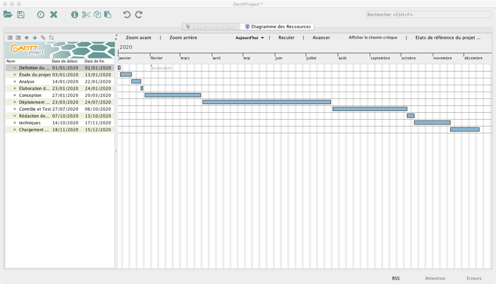
\includegraphics[width=14cm]{ganttt.png}
	\caption{Diagramme de Gantt.}
	\label{fig:mvc}
\end{figure}

\subsection{Contraintes du projet}

\underline{Contraintes de sécurité.}

La gestion de la sécurité est la principale contrainte de notre système. L’application doit posséder une gestion de privilèges et niveaux d’accès pour les différents types d’utilisateurs. Selon leur statut, le contenu des pages varie et l’accès aux informations avec un statut supérieur est interdit.

\underline{Autres contraintes techniques}

Pour le développement de notre système, nous disposons d’une architecture existante sur laquelle nous devrons baser notre application. La structure de notre systéme doit être extensible. De plus, le développement devra suivre toutes les normes techniques pour une meilleure performance, maintenance et facilité de mise à jour.

\section{Méthodologie de conduite de projet.}

\subsection{Modèle de cycle de vie en cascade\cite{Ref13}}

Mis au point dès 1966, puis formalisé vers 1970, le cycle de vie de projet en cascade est un type de cycle de vie, simple à comprendre et à implémenter, convient aux projets où la qualité a plus d’importance que les coûts ou les délais, et dont les besoins sont clairement définis et stables. Dans le cas contraire, la prise en compte de nouveaux besoins nécessite de dérouler toute la cascade depuis le début. De plus, le client n’est impliqué qu’au début du projet et il ne peut tester le produit qu’à la fin du processus. Dans le cadre d’un projet de gestion des identités et des accès, les besoins peuvent évoluer. En effet, le déploiement de nouveaux services implique notamment la définition de nouveaux profils ainsi que de nouveaux rôles applicatifs qui doivent être pris en compte, même après la phase de spécification. De ce fait, ce modèle de gestion de projet ne convient pas à notre projet.

\begin{figure}[H]
	\centering
	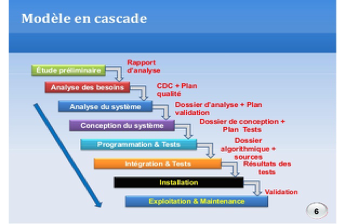
\includegraphics[width=14cm]{cascade.png}
	\caption{Modèle de cycle de vie en cascade}{ \begin{center} source :\textit{Google} \end{center}}
	\label{fig:cascade}
\end{figure}

\subsection{Modèle de cycle de vie en V\cite{Ref13}}

A l’instar du modèle en cascade, celui en V prend difficilement en charge de nouveaux besoins ou la modification des spécifications. En effet, l’effet tunnel induit par les modèles séquentiels montre qu’une erreur dans la formulation ou l’interprétation des spécifications ne peut être détectée qu’a la fin du cycle. La maitrise d’ouvrage n’est impliquée qu’en début et fin de cycle, ce qui peut représenter plusieurs mois d’intervalle pour un gros projet. Bien plus nombreuses que dans un cycle en V, les possibilités de prise en compte de nouveaux besoins restent faibles. En effet, dans le cadre de notre projet, après la phase de spécification, la mise à disposition d’un nouveau service, ne peut être prise en compte qu’au moment des tests d’intégration. De plus, ces changements impliqueraient la remise en cause du travail effectué jusqu’à la phase des tests unitaires.

\begin{figure}[H]
	\centering
	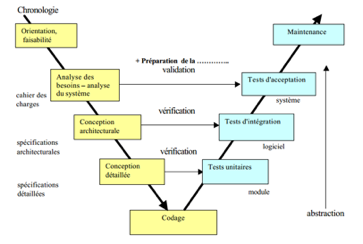
\includegraphics[width=14cm]{V.png}
	\caption{Modèle de cycle de vie en V}{ \begin{center} source :\textit{Google} \end{center}}
	\label{fig:V}
\end{figure}

\subsection{Modèle de cycle de vie en spirale \cite{Ref13}}

Représenté à l’aide d’une spirale et proposé par Boehm en 1988, ce modèle est beaucoup plus général que le précédent. Chaque boucle de la spire représente une phase du développement celle la plus interne traite des premières phases. La plus externe traite de la livraison, chaque boucle traverse quatre sections :

	\begin{itemize}[label=\textbullet, font=\LARGE \color{blue}] 
		
		\item Définition des objectifs de la phase 
		\item Évaluation des risques et plan de gestion
		\item Développement et validation
		\item Planification de la phase suivante
	\end{itemize}
	
	Le fait qu’il soit un méta-modèle entraine l’obligation de l’instanciation de chaque boucle, création d’une boucle de faisabilité, d’une boucle de prototypage, des boucles de développement itératif, etc.
	
De ce fait, il faut alors trouver le bon modèle de processus pour chaque boucle.

\begin{figure}[H]
	\centering
	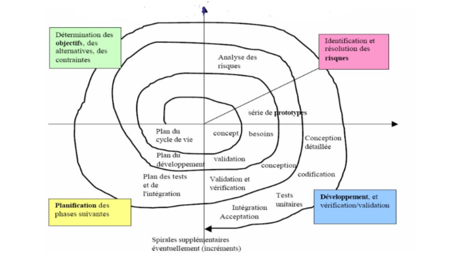
\includegraphics[width=14cm]{spirale.png}
	\caption{Modèle de cycle de vie en spirale}{ \begin{center} source :\textit{Google} \end{center}}
	\label{fig:spirale}
\end{figure}

\subsection{La méthodologie agile \cite{Ref1}}

Adopter les méthodes agiles constitue un acte courageux car il s’agit de quitter un système organisationnel, culturel et économique connu (étudié en cours et utilisé tout au long de la formation) pour s’orienter vers l’inconnu avant d’atteindre à nouveau un équilibre stable. Les raisons qui nous poussent à adopter une méthode agile sont nombreuses et variées. La capacité à s’adapter au changement, à livrer plus fréquemment et à accroitre la qualité des logiciels ainsi développés figurent parmi les motivations les plus fréquentes. La bonne surprise réside dans le fait que la motivation des équipes est également une raison très souvent citée. Preuve est ainsi faite que les méthodes agiles représentent un système de valeurs et sont perçues par un grand nombre comme un changement culturel motivant, bénéfique pour tous. 

L’agilité ou plutôt les méthodes agiles sont un groupe de processus et de pratiques pour le pilotage et la réalisation de projets. Toutes ces pratiques sont basés sur le manifeste agile, qui a été mis en place en 2001 et qui a pour but d’impliquer au maximum le client, ou bénéficiaire du projet, dans le développement, pour permettre une réactivité dans la réalisation de ses demandes. 

\begin{figure}[H]
	\centering
	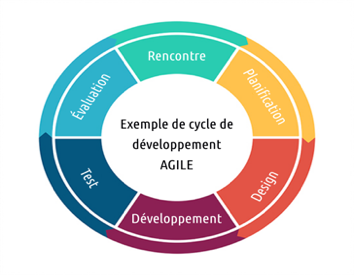
\includegraphics[width=14cm]{methode_agile.png}
	\caption{Méthode agile.}{ \begin{center} source :\textit{Google} \end{center}}
	\label{fig:mvc}
\end{figure}

\subsection{Pourquoi la méthodologie agile}

La motivation de notre choix sur la méthode agile est contenue dans le tableau ci-dessous. Qui présente les principales différences entre les approches classique et les approches traditionnelles. Ces différences sont organisées par thèmes, lesquels correspondent aux principes du manifeste.


\begin{table}[H]
	\caption{Méthodes : agiles vs classiques.\cite{Ref8}}
	\label{Méthodes : agiles vs classiques.}
	\centering
	\begin{tabularx}{\linewidth}{|X|X|X|}
		\hline \rowcolor{lightgray}  
		\textbf{Thème} & \textbf{MÉTHODES AGILES} & \textbf{MÉTHODES CLASSIQUES}\\
		\hline
		Objectif & Satisfaire l’utilisateur &  Respecter le besoin initial et les engagements\\
		\hline
		Changement & Accepter le changement &  Opposé au changement ou, en tout cas, moins enclin à l’accepter compte tenu des livraisons tardives et des processus de gestion lourds\\
		\hline
		Livraison & Livrer fréquemment  & Livrer en une seule fois une application « finalisée »\\
		\hline
		Équipe  & Travailler en synergie &  Travailler de façon segmentée (chacun voit sa partie du travail) \\	
		\hline
		Moteur & Stimuler la motivation  & Stimuler la productivité\\
		\hline
		Communication  & Communiquer en direct avec les opérationnels & Communiquer de façon verticale en passant par
		des relais hiérarchiques (par exemple, le chef de projet MOE est relais entre la MOA et ses développeurs)\\
		\hline
		Indicateurs &Un seul indicateur : les fonctionnalités
		implémentées & Justifier par les indicateurs (sans livraison
		intermédiaire, les indicateurs sont les seuls
		justificatifs de l’avancement, des écarts, etc.) \\
		\hline
		Rythme & Bannir les rushs de production & Adapter la production aux contraintes projets \\
		\hline
	%	Qualité & 	\multicolumn{2}{|X|}{	 Que ce soit en méthode agile ou classique, l’excellence technique est essentielle. Ce neuvième principe sert principalement à justifier le fait que les méthodes agiles prônent la qualité des livrables techniques (contrairement à ce que peuvent en dire un certain nombre de détracteurs) }\\		\hline
			Livrables &Rester concentré sur l’essentiel			(la production) & Une documentation précise est essentielle pour assurer les échanges et la validation autours des besoins client \\
		\hline
			Autonomie & Favoriser une certaine autonomie
			des équipes & Encadrer scrupuleusement le travail
			des équipes \\
		\hline
			Rythme & Intégrer la notion d’amélioration continue
			tout au long du projet & Introspection possible mais uniquement en fin
			de projet \\
		\hline
		
	\end{tabularx}
\end{table}{  source : \textit{https://www.consultrade.info/gestion-de-projet/la-gestion-de-projet-methode-classique-vs-agiles/}